\section{Solution Juniper/Pulse}
La solution de Juniper se base sur l'utilisation d'une passerelle SSL.
Celle-ci gère les connexions entrantes, et attribue, aux connexions autorisées, l'accès aux ressources.
La passerelle utilisée est une SA 2500 tournant sous Pulse Connect Secure 8.1R1.1.
Les clients distants peuvent se connecter soit via le portail Web, soit via le client Pulse Secure.

Le client Pulse Secure est fourni par la passerelle.
Cette dernière peut distribuer le software à tous les utilisateurs authentifiés automatiquement ou en le téléchargeant via le portail Web.

\subsection{Schéma de l'infrastructure}
Comme la passerelle est accessible depuis l'extérieur, elle ne possède pas le même niveau de confiance que le LAN.
Elle est donc placée dans une DMZ (voir Fig.\ref{fig:schemaJuniper} p.\pageref{fig:schemaJuniper}).
\begin{figure}[ht]
	\centering
	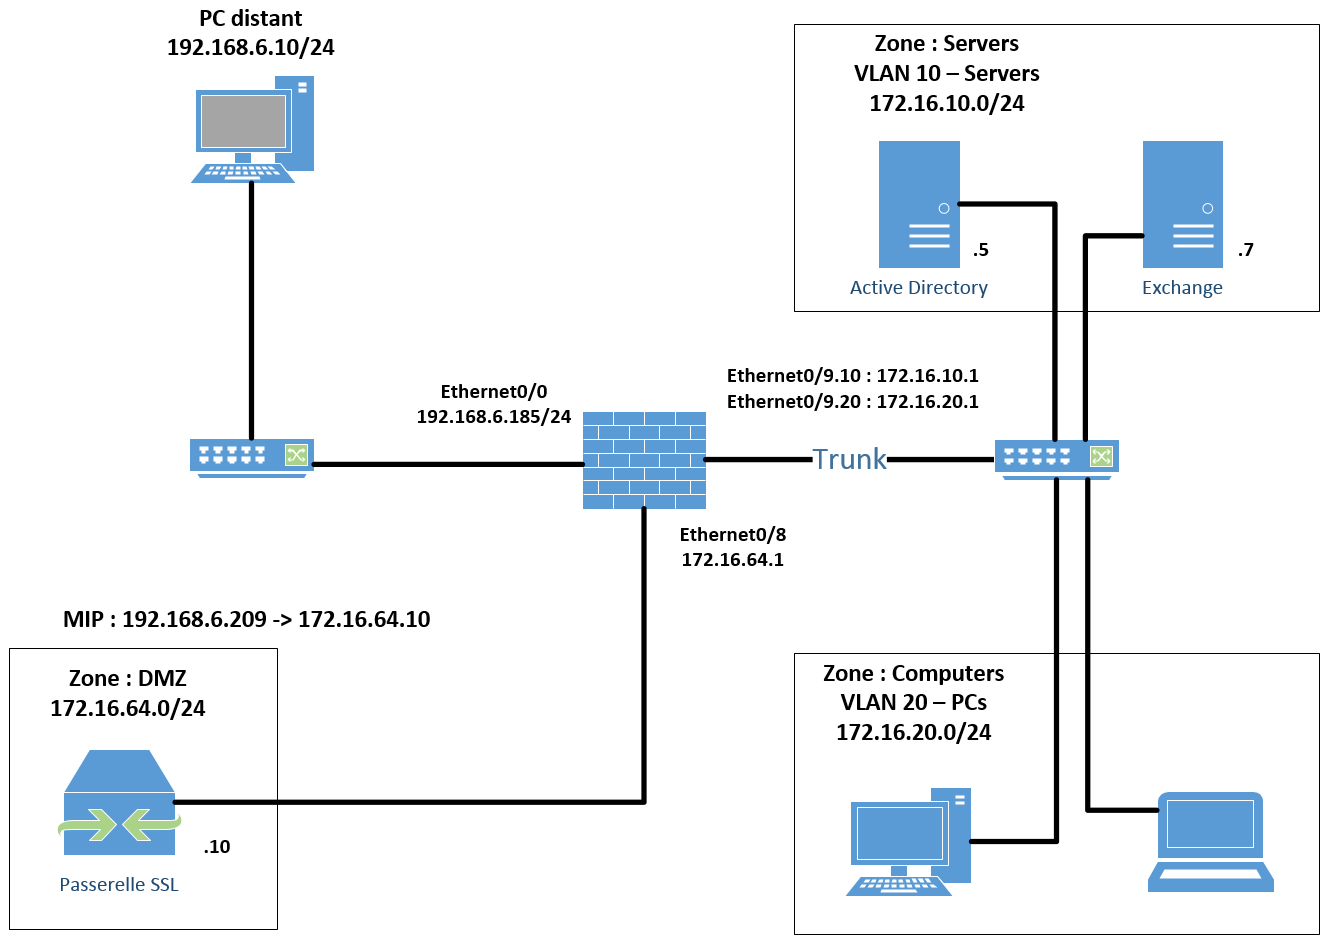
\includegraphics[width=16cm]{juniper/schema.png}
	\caption{Schéma logique de l'infrastructure}
	\label{fig:schemaJuniper}
\end{figure}

Le firewall sert de routeur entre le réseau du labo (externe) et le réseau de test (interne).
Il gère aussi les \textit{policies}, c'est-à-dire les règles entre les zones de sécurité établies dans la configuration.
Dans mon réseau de test, j'ai créé deux zones en plus de celles pré-définies : la zone "Computers" et "Servers".

Pour l'adressage (Fig.\ref{fig:ifJuniper} p.\pageref{fig:ifJuniper}), ma zone \textit{Untrust} est le labo. 
L'interface associé possède l'adresse 192.168.6.185.
Les autres zones font parties du réseau de test et possèdent une adresse dans le réseau 172.16.0.0/16.
J'utilise les VLAN 10 et 20 pour différencier le trafic des ordinateurs et des serveurs sur le même interface.
L'utilisation de deux zones distinctes est une bonne pratique avec Juniper. 
Il est plus claire de créer des \textit{policies} entre des zones, que de créer des ACL sur les interfaces.
\begin{figure}[ht]
	\centering
	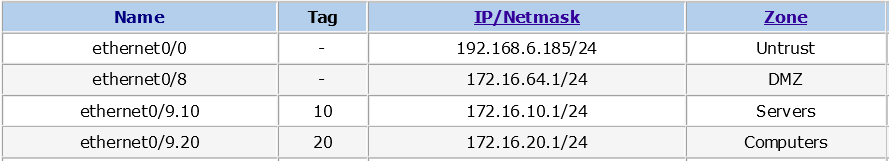
\includegraphics[width=16cm]{juniper/interfaces.png}
	\caption{Adressage des interfaces}
	\label{fig:ifJuniper}
\end{figure}

Pour autoriser l'accès à la passerelle, l'utilisation d'un mappage est indispensable.
On a mappé l'adresse externe (192.168.6.209) avec l'adresse de la passerelle dans la DMZ (172.16.64.10).
Le mappage ne suffit pas, il faut aussi autoriser le trafic entre la zone \textit{Untrust} et la DMZ (Fig.\ref{fig:polUnDMZ} p.\pageref{fig:polUnDMZ}).
En suivant les règles de bonnes pratiques, j'autorise uniquement le trafic HTTPS et ESP entre un client en remote-access et la passerelle et je bloque tous les autres trafics.
\begin{figure}[ht]
	\centering
	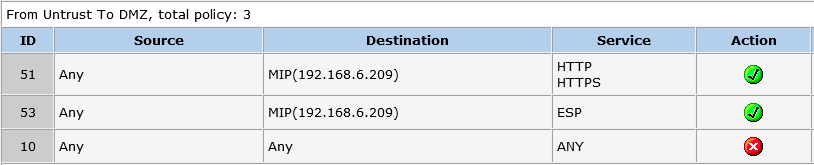
\includegraphics[width=16cm]{juniper/Policy-Untrust-DMZ.png}
	\caption{Policies entre la zone Untrust et la DMZ}
	\label{fig:polUnDMZ}
\end{figure}

\subsection{Configuration de la passerelle  SSL}
\subsubsection{\textit{Realm} et rôles}
Pour commencer, on définit le \textit{realm} d'authentification.
Il existe plusieurs possibilités, j'ai choisi d'utiliser une authentification simple via l'Active Directory.
Ce mode d'authentification est fiable, mais pour une sécurité renforcée, il est intéressant de passer à une double authentification.
La double authentification s'active en cochant l'option dans la configuration du \textit{realm} (voir Fig.\ref{fig:confRealm} p.\pageref{fig:confRealm}).
\begin{figure}[ht]
	\centering
	\includegraphics[width=16cm]{juniper/Authserv.png}
	\caption{Configuration du \textit{realm} d'authentification}
	\label{fig:confRealm}
\end{figure}

À chaque realm, on mappe l'utilisateur à un rôle.
Dans mon cas, mes utilisateurs appartiennent soit au rôle "It Tech", soit au rôle "All Employee".
Cette attribution dépend du groupe Active Directory auquel appartient l'utilisateur (voir Fig.\ref{fig:mapRoles} p.\pageref{fig:mapRoles}). 
\begin{figure}[ht]
	\centering
	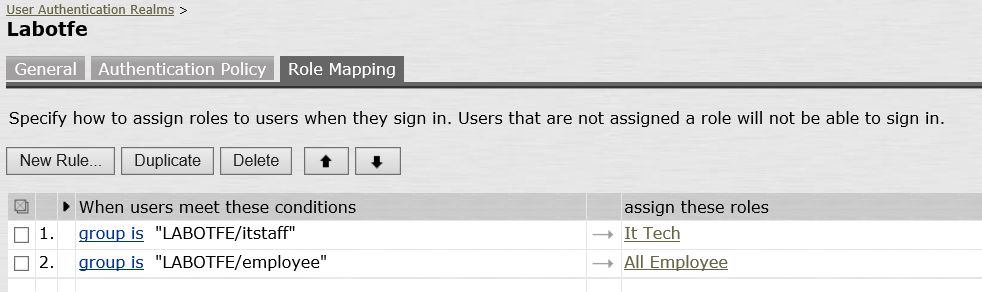
\includegraphics[width=16cm]{juniper/Rolemapping.png}
	\caption{Mappage des rôles dans le realm}
	\label{fig:mapRoles}
\end{figure}

À ces deux rôles, j'ai associé des ressources différentes (voir Fig.\ref{fig:resRoles} p.\pageref{fig:resRoles}).
\begin{figure}[ht]
	\centering
	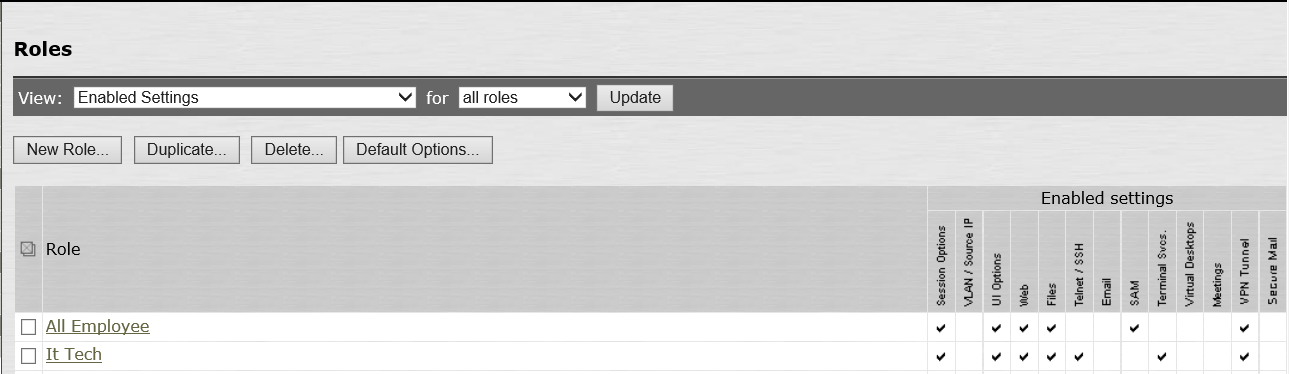
\includegraphics[width=16cm]{juniper/UserRoles.png}
	\caption{Ressources associées aux rôles}
	\label{fig:resRoles}
\end{figure}

\subsubsection{VPN - Portail Web}
Le portail Web se configure en créant une "Sign-in Pages".
Les utilisateurs distants y accèdent via un navigateur web.
Pour une sécurité accrue lors de l'accès à cette page, j'ai activé le "Host Checker".
Il permet de vérifier des propriétés de la machine du client pour autoriser l'accès à la "Sign-in Page".
Dans ce cas-ci, l'"Host Checker" vérifie l'appartenance au domaine \textit{labotfe.be}. 

Une fois la vérification du nom de domaine effectuée, l'utilisateur peut saisir ses identifiants sur le portail.
Le portail permet au client d'accéder aux ressources, qui sont attribuées à son rôle.
Les ressources accessibles sont définies sur la passerelle SSL en tant que \textit{bookmarks} (voir Fig.\ref{fig:bookmarks} p.\pageref{fig:bookmarks}).
\begin{figure}[ht]
	\centering
	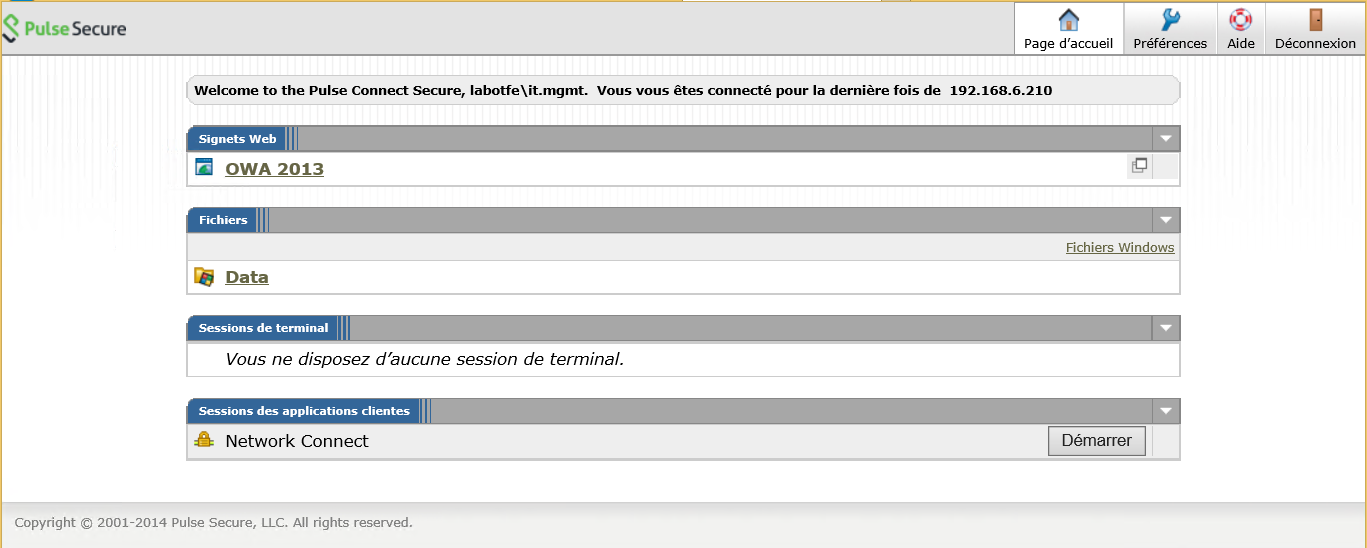
\includegraphics[width=16cm]{juniper/portail.png}
	\caption{\textit{Bookmarks} associés à un membre du groupe It Tech}
	\label{fig:bookmarks}
\end{figure}

\subsubsection{VPN - Pulse Secure}
Une fois le client installé, l'utilisateur saisit ses identifiants dans la fenêtre de Pulse Secure. 
La connexion se fait automatiquement. 
Pour une question de sécurité, la passerelle essaie d'établir une connexion en ESP et elle peut passer en SSL en cas d'échec de la connexion ESP.
L'ESP se fait en encapsulant les paquets dans un paquet UDP sur un port précis.
Mais si ce port est bloqué à un endroit entre le client et la passerelle, la connexion ESP est impossible.
L'option de fallback peut être désactivé pour améliorer la sécurité. 

Comme les utilisateurs ont un rôle assigné, on définit à chaque rôle un espace d'adressage sur la passerelle pour les utilisateurs (voir Fig.\ref{fig:profilVPN} p.\pageref{fig:profilVPN}).
Ainsi le rôle "It Tech" possède les adresses de l'espace 172.16.64.192/27 et le rôle "All Employee" celle de l'espace 172.16.64.224/27.
De cette manière, on peut gérer les accès au niveau du firewall de façon granulaire, c'est-à-dire en autorisant seulement certaines adresses à accéder à certaines ressources.
\begin{figure}[ht]
	\centering
	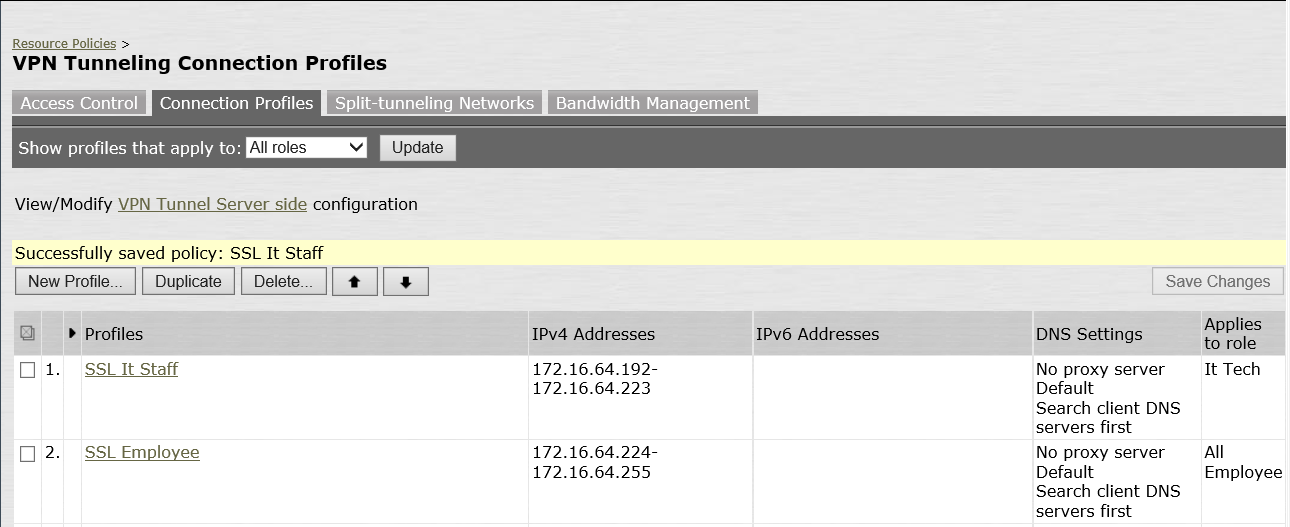
\includegraphics[width=16cm]{juniper/VPNProfiles.png}
	\caption{Profils VPN}
	\label{fig:profilVPN}
\end{figure}